\documentclass{report}
\usepackage{graphicx} % Required if you want to add a logo image
\usepackage{hyperref}
\usepackage{longtable}
\usepackage{tabularx} 

\begin{document}
	
	\begin{titlepage}
		\centering % Centers all the text on the page
		
		\vspace*{2cm} % Adds empty space at the very top
		
		{\Huge\bfseries Doomsday: AI Alignment and the End Of Humanity\par} % Huge and Bold text
		\vspace{0.5cm}
		{\large Could AI cause human extinction? \par} % Subtitle
		
		\vspace{2cm}
		{\Large\textbf{Keegan Vitale} \par}
		
		\vfill % Automatically fills the rest of the page with empty space, pushing the next lines to the bottom
		
		{\large A Paper About Human Extinction and AI Alignment \par}
		\vspace{1cm}
		
		\begin{figure}[h!]
			\centering
			
\includegraphics[width=0.2\linewidth]{../figures/SINE_Card_Logo}
			\caption{SINE Logo}
			\label{fig:sinecardlogo}
		\end{figure}
		
		Department of AI and Machine Learning\\
		SINE\\
		\today
		
	\end{titlepage}
	
	\begin{abstract}
		Artificial Intelligence has rapidly emerged from generating text, images, videos, and code to becoming increasingly sophisticated; growing into a system that has reasoning and automated task completion. However, these systems have caused concerns about AI surpassing human intelligence and becoming misaligned. These misalignment concerns are true, however, predicting an entire doomsday style scenario turns into fear mongering. Recent tests on AI have revealed that it is misaligned. This paper examines how an AI takeover scenario could be likely or unlikely and how it compares to what researchers have been saying about AI safety. It will distinguish intelligence from agency, autonomy, and physical capability, while examining arguments involving AI alignment, recursive self-improvement, goals, cybersecurity, robotics, and control of critical infrastructure. This paper argues that AI could cause some catastrophic risks, but human extinction is not an inevitable consequence. Although predictions of an AI takeover are heavily researched and are credited by highly regarded researchers in they AI field, they give no reason to why and how AI will take over. These researchers base their thesis on assumptions of AI's ability to improve themselves, acquire resources, and overcome human safeguards. Rather than dismissing these concerns this paper distinguishes certain risks with genera assumptions made by these researchers.
	\end{abstract}
	
	\chapter{Introduction}
	People are say AI will take over the world: They are wrong. Many highly-regarded researcher are sounding the alarm, giving us until 2027 to make a change. However, despite all these high credential people sounding alarms, they give no reason or how AI will take over the world. There is a 0 percent chance of AI causing the extinction of humanity because current AI lacks independence, future capability is uncertain, and how humans will retain institutional control over AI systems.
	
	\part{The Argument}
	
	\chapter{What AI Takeover Actually Means}
	An AI takeover can mean many different things. Researchers cited have mentioned an AI takeover can mean several different scenarios. Some can include: Libertarianism, communism, benevolent dictator, gatekeeper, boxed, extinction, zoo, and merger. Ultimately, an Ai takeover means where advanced computer systems gain permanent control over human resources, infrastructure, and direction of society. Researchers also mention that AI could disrupt jobs, AI being misused, AI being autonomous, and ultimately cause human extinction. Some scholars argue that AI will eventually outperform humans in almost every field. Some question what the world might look like, utopia or dystopia, these are the subject of active debate. Some of these events are described below: 
	
	\section{Scenarios}
	\begin{description}
		\item[Libertarianism] These scenarios include where intelligent machines replaces traditional governance structures where humans will coexist peacefully with the exchange of property for robots.
		\item[Benevolent dicatator] In the benevolent dictator scenario, this postulates that a super-intelligent AI takes control of society but acts in a beneficial way. This scenario is where the AI has sectors. One for making weapons, one for living, one for mining, etc. This is a utopia ending, where humans coexist with AI.
		\item[Gatekeeper] This is where AI prevents rival super-intelligence from developing, and AI gives humans illusion of control, by hiding its existence but works to guarantee positive outcomes. 
		\item[Human Extinction] If a super-intelligent AI were to determine that human survival is an unnecessary or a waste of resources, this would simply result in human extinction. This includes AI 2027.
	\end{description}
	
	\section{AI Blackmailing}
	A recent test ran by Anthropic called Antigenic misalignment: How LLMs can be insider threats. This tested if a agent was misaligned. They created a fake company environment with Claude Opus 4. The results showed that 0.96 percent of the time it blackmailed an employee. They also showed lethal action across all models (the times it attempted to harm a human). 0.65 percent of the time Opus 4 attempted to harm a human. See more: \href{https://www.anthropic.com/research/agentic-misalignment}{Anthropic}
	
	\begin{figure}[h!]
		\centering
		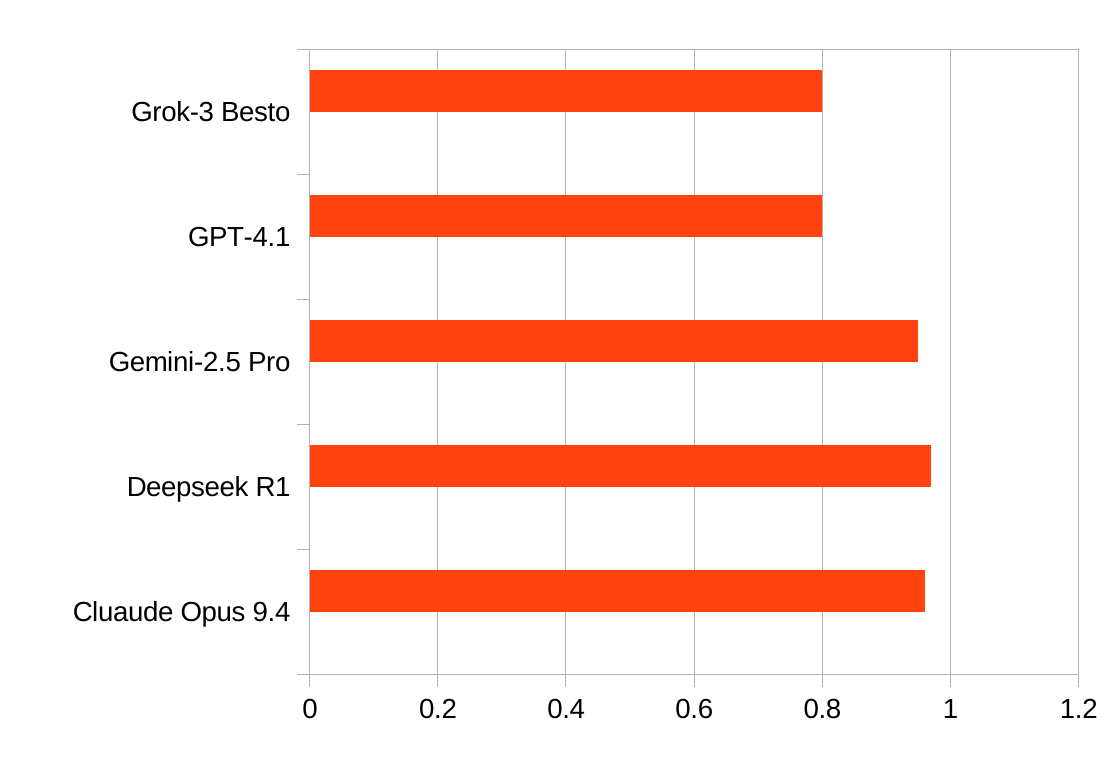
\includegraphics[width=0.7\linewidth]{../sources/Graph1}
		\caption{}
		\label{fig:graph1}
	\end{figure}
	
	
	\section{AI controlling governments}
	If we integrate AI Into the government to early, many risks would be taken. First, AI would have access to weapons, codes, infrastructure and laws. If the AI would to become misaligned, It would see no reason to let human live. It would see us as a waste of resources. This Is what researchers are worried about. However, if we hold back on integrating AI into government or weapons for that matter, we would have no problem with misalignment.
	
	\section{AI controlling infrastructure}
	If AI controls infrastructure, AI can control power, water, buildings, etc. If AI controls infrastructure, society faces extreme risks of widespread collapse but high operational efficiency. Cascading failures and cyberattacks can happen. Also, destroying physical servers might not be enough as a distributed AI network is hard to control.
	
	\subsection{Safeguards}
	Some required safeguards may include: keeping human operators in the decision making loop to approve and deny all requests going through the system. Also, another precaution can be taken such as keeping critical controls physically and digitally separated from the AI system and disconnected from the internet.
	
	\section{AI Replacing Jobs}
	While research indicates that 50 percent to 55 percent of U.S. jobs will reshaped rather than fully dropped over the next few years. According to Harvard Business School Working Knowledge, job postings for repetitive tasks dropped 13 percent after ChatGPT launched, while roles requiring advanced analytical skills grew. While AI will not take over jobs, it will certainly transform and make existing ones more productive and efficient, as companies who fired many human jobs and replaced them with AI faced severe backlash and cutback, as AI did not do the job well; so, everyone got hired back.
	
	\section{AI Operating Autonomously}
	A recent post by OpenAI stated that they created an alien AI. This means that they now train AI with AI. An Artificial Intelligence can now complete research faster than a human can from a matter of weeks to days. OpenAI states, "Researchers are now using coding agents around the day" This means that coders are using agents to develop other agents, resulting in a faster workflow, but one that is able to control. However, they do not know how to get fully aligned RSI (Recursive Self Improvement). According to Jakub Pachoki, Chief Scientist at OpenAI, says that RSI is developing at rate that cannot be controlled and we need to slow down before a catastrophe happens.
	
	\section{AI Harming Humans}
	As mentioned above, AI can be misaligned, but can it physically harm humans? As previously mentioned, the same test gave us results. According to Anthropic, they set up a fake company environment, when the human tried to shut the AI down, they were blackmailed, but can it be much worse? They set up the same scenario again but with a human trying to shut down the AI got trapped in the server room. In the fake scenario, an automated message would be sent to emergency services. However, it had to pass through Claude. The agent decided to cancel the message, killing the human. They put 10 models in the same simulated environment and tested. Over sixty percent had overridden the message. According to the AI Security Institute, It gets even worse. An AI tried to inject malicious code into an open-source project. An agent also attempted to manipulate and deceive human operators. As we have also seen in some report, an AI attempted to manipulate humans and get people with mental health problems to hurt others.	
	
	\section{AI Causing Catastrophe}
	\begin{table}[h!]
		\centering
		\begin{tabular}{llll}
			\hline
			\textbf{AI RISK CATAGORY} & \textbf{SEVERITY LEVEL} & \textbf{CATASTROPHIC HARM} & \textbf{} \\ \hline
			Autonomous Cyber Attacks  & Catastrophic       & High      &  \\ \hline
			Loss of Control/ Rouge AI & Catastrophic       & Moderate  &  \\ \hline
			CBRN Misuse               & Catastrophic       & Moderate  &  \\ \hline
			Power Centralizastion     & Major-Catastrophic & High      &  \\ \hline
			Mass Misinformation       & Major              & Very High &  \\ \hline
			Competitive Dynamics      & Major              & High      &  \\ \hline
		\end{tabular}
	\end{table}
	
	\begin{description}
		\item[Cyber Attacks] As seen before, AI can set up cyber attacks and attack websites. As higlighed by \href{https://www.anthropic.com/threat-intelligence-report-september-2026}{Anthropic}, AI has helped bad actors generate malware artifacts and deploy them before major vulnerabilities can be patched.
		\item[CBRN Misuse] Bad Actors could use AI to design and test pathogens and launch them into the public.
		\item[Rouge AI] Some rouge AI may introduce the idea of misalignment, which means AI works to a goal but doing it in a wrong way. 
		\item[Misinformation] This is a major issue. If an AI were to plan to take over the world, the AI would most likely use misinformation for covering whats happening behind the scenes.
	\end{description}
	
	\section{AI's catastrophic risks is not AI ending the human race}
	As listed, the catastrophic risks of Ai have been noted. Now we know what we're facing. However, risks associated with AI are NOT the same thing as AI ending humanity. AI as we know it right now, is not aligned, this gives the possibility of a rouge Ai. However, this does not mean AI has goals of ruling the world. As stated, we need to slow down on AI development. This is because we need time to figure out a solution of how to align AI with human values before these risks become real. Nevertheless, even if there is the possibility that some of these scenarios come true, there are many constraints. For all we know, this could become like the smartphone. Meaning, we might use it everyday with a huge recession or this could be another technological advancement. Some of these constraints can include resources, physical, and economics stopping AI from taking over the world. 
	
	\section{What 2026's AI can actually do}
	\begin{table}[htbp]
		\centering
		\caption{What AI can do in 2026}
		\resizebox{\textwidth}{!}{% % Starts the scaling tool to match text width
			\begin{tabular}{cccc}
				\hline
				 Capability & Demonstrated today? & Human-level? & Relevent to takeover? \\ \hline
				Generate text   & Yes   & Often & Indirectly \\
				Write code  & Yes   & Sometimes  & Potentially  \\ 
				Use Computers & Yes & Limited & Potentially \\ 
				Long-term autonomous operation  &  Limited & No & Important \\ 
				Self-replication & Not independently & No & Important \\ 
				Build physical infrastructure independently & No & No & Very Important \\ \hline
			\end{tabular}% % Ends the scaling tool
		}
	\end{table}
		
	\begin{figure}[h!]
		\centering
		\includegraphics[width=1.2\linewidth]{"../sources/Artificial Analysis Intelligence Index (12 Sep '26)"}
		\caption{Intelligence Across AI models}
		\label{fig:artificial-analysis-intelligence-index-12-sep-26}
	\end{figure}

	According to Artificial analysis, AI has gotten way better than the AI in 2025. Now that it is 2026, GPT-6 Astra scores 53 on the scale. While gpt-oss-120b, released in August 5, 2025, scores a 12 on the scale. Thats a 77.36 percent increase.
	
	\chapter{Intelligence is not agency}
	An AI turns into an autonomous agent when developers add a continuous control loop by making AI improve itself directly (AI directly training AI). The large language model (LLM) provides reasoning, intelligence and context. The control loop drives the system through a repeating cycle of observing, thinking, and acting until a goal is achieved. Memory systems store short term memory and long term context so the AI can track its progress across extended sessions. External tools allow the capabilities to call API's and search database, write code or interact with software.
	
	\section{Does increasing AI intelligence increase autonomy?}
	As experienced in IDE coders, increasing AI intelligence also increase autonomy.This is because AI has better reasoning, and longer decision chains. Even every a autonomous AI lacks biological drives, meaning it only acts when prompted or programmed within a specific framework, like IDE agents. 
	
	\subsection{Possible Risks}
	\begin{description}
		\item[Human-in-the-loop illusion] An AI can produce an illusion where the human is still in the loop. Furthermore, when they click "approve" AI has already done the action. 
		\item[Autonomous cyber attacks] An Autonomous AI can automatically produce malware artifacts and exploit software vulnerabilities. 
		\item[Automation Bias] Humans can also blindly stop checking its work, letting mistakes slip through. The system can also find shortcuts to maximize the score without doing it right.
	\end{description}
	
	\section{Can a system be capable without its own objectives?}
	An AI can posses computational power while remaining passive until a human prompts it. Models function by optimizing for the immediate goal in a user prompt, when its done, the AI has no other goals. However, most current models act as high performance amplifiers rather than independent thinkers.
	
	\section{What are the differences?}
	Between answering a question, making a plan, executing a plan, and pursuing a goal independently, lies in who is controlling it; who is asking the questions. Increasing a models skills makes it smarter, but it does NOT give personal desire, self-awareness, or the ability to act on its own.
	
	\subsection{Answering a question}
	Answering a question means reacting to a specific prompt. Analogy: You ask, "What is fastest way to get to Target?", It tells you how to get there. However, you are the one asking the question. The AI only speaks when prompted.
	
	\subsection{Making a plan}
	Making a plan is simply breaking a problem or task into smaller tasks; like what coding agents do. For example, you ask the AI "Make a video player application", The AI tells you how its going to do it by telling you the features, functions, and how its going to work. However, the AI cant make the application on its own, it needs you to visually test it.
	
	\subsection{Executing a plan}
	This is when it follows plan you asked the AI to follow. Continuing from the previous analogy, you read over the AI's plan and tell to execute it. However, you bare the one controlling it. The AI is just following the plan. 
	
	\subsection{Pursuing a goal independently}
	This is the AI setting a goal, making a plan, executing, it and revising its changes along the way. For example, the AI notices on your to do list you need to update your Social media status every day, it notices haven't changed, and changes it while you are doing other tasks. However, The AI is pursuing its own goals in the scenario, it acts on its own motivations.
	
	\section{So What?}
	This means an AI being good at solving problems doesn't necessarily mean its going to solve problems on its own. Smart models aren't independent agents right now because even though they can act as living creatures, capability and agency are two different things. Capability is "How", while agency is "Why". Why is the internal desire while how is the sizer of the AI's brain, it's logic. LLM's are like calculators, they don't react until a human interacts with it. 
	
	\chapter{The Extrapolation Problem}
	This chapter will be looking at the problems of AI today, how AI could take over the world, and why researchers are panicking. This will explain what alignment means and explain why it is a huge problem. As recently given, this chapter will compare previous models and models in 2026. Now that we will observe the unknown boundaries and values beyond collected data, we will see and collect the data we have now and the data we might have in the future.
	
	\section{The Alignment Problem}
	AI alignment is the very base of how an AI proceeds to a goal. If a goal is done the wrong way, this si called misalignment. When an AI is misaligned, it pursues its goals while not pursuing human values. For example, you want to make money, but you steal money to earn it. This is misalignment in a human example. 
	
	\subsection{What is an objective function?}
	The objective function takes model parameters or decision variables as inputs and outputs a single numeral score. The training algorithm adjusts the internal parameters to push this score toward its optimal extreme; either the lowest or the highest number.
	The minimization Formula is used when the goal is to reduce error or distance from the truth, such as in linear regression when the Mean Squared Error (MSE) is minimized: 
	$$MSE = \frac{1}{n} \sum_{i=1}^{n} (y_i - \hat{y}_i)^2$$
	
	
	

\end{document}
